\documentclass[12pt,fleqn]{article}\usepackage{../common}
\begin{document}

\begin{minted}[fontsize=\footnotesize]{python}
import pandas as pd
df = pd.read_csv('CountryAverageDataPilotStudy.csv',index_col='year')
df = df[(df['name']=='Nigeria')]
df[['meanW']].plot()
plt.savefig('test_01.png')
\end{minted}

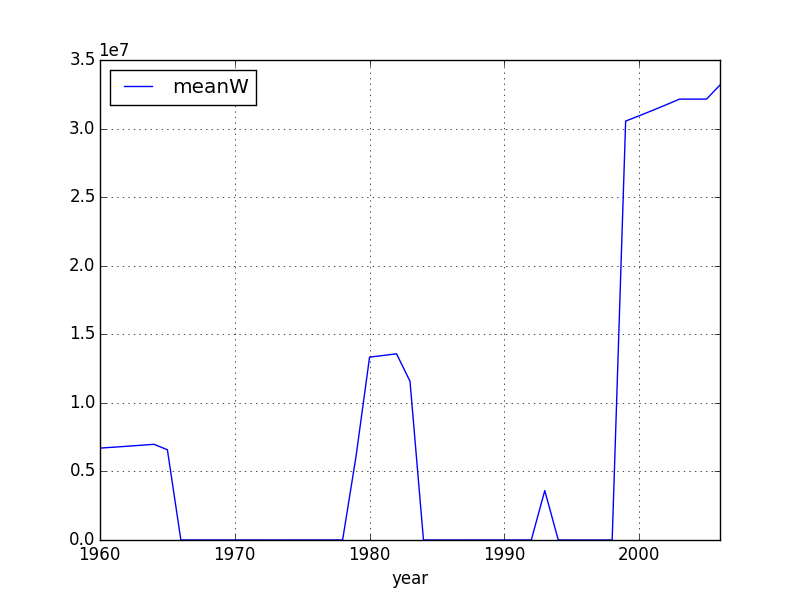
\includegraphics[height=6cm]{test_01.png}

\begin{minted}[fontsize=\footnotesize]{python}
df[['meanS']].plot()
plt.savefig('test_02.png')
\end{minted}

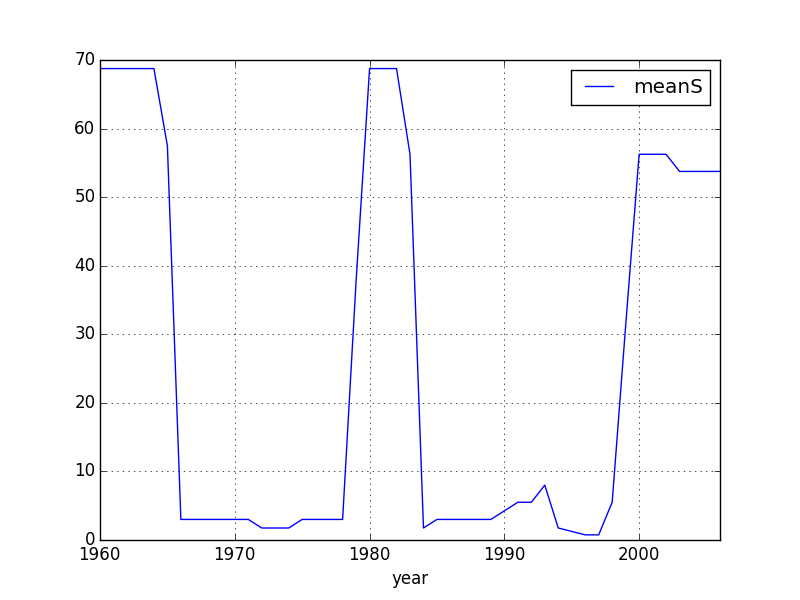
\includegraphics[height=6cm]{test_02.png}





\end{document}
